%\setcounter{page}{0}
\chapter{1. Introduction}

\section{From Drive-less Cars to Car-less Cities}
\setcounter{page}{1}
The challenge of moving people and goods around the world's dense, growing major cities is hard and getting worse. Nearly ninety per cent of the world's population growth will be concentrated in Asia and Africa, and is expected that 2.5 billion people will add to the world's urban population by 2050. Furthermore, cities will soon account for 80 percent of global carbon emissions, according to the United Nations urbanization prospects.\cite{UnitedNations2014}  

Much of that emissions will come from idling cars stuck in kilometers-long traffic jams. Cities around the world are striving to improve livability by way of reducing dependency on fossil-fuel vehicles, applying controversial policies and restrictions, usually not understood by the citizens. Hence, for the moment no key solution has been found. In fact, this problem is much more complex and will require long-term solutions. 

In this way, technology is evolving to address better urban transportation, more secure and environmentally friendly urban transportation. In the coming decades, the transportation world will be totally transformed by three concepts: \textbf{Electrification, autonomy and shared economy.}

\newpage
\subsection{Electrification}

The immediate way of getting rid of the pollution that internal combustion engines produce is to install electric motor based drive-trains in our cars, which account for the most percentage of the emissions. 

The introduction of a fully electric transportation system will need new infrastructure, charging stations and more capacity in the electrical grid.
However, it is undeniable that with the exhaustion of fossil fuels, electric vehicles will replace current cars in the near future. The appearance of hybrid propulsion systems supposes the first step towards the electrification.
While it is clear that at the moment electric vehicles present some limitations, such as battery range, the development of energy storage technologies will get over these issues in the next years.

\subsection{Autonomy}

Nowadays, self-driving vehicles are almost a reality, thanks to the improvements in artificial intelligence and computer technologies. 

On one side, the development of new techniques and algorithms in artificial intelligence have expanded the capabilities of conventional cars. Deep learning techniques, along with artificial neural networks have been able to achieve high levels of autonomy by using data coming from different sensors -- \textit{cameras, ultrasonic, radar and lidar} -- that give enough information about the car's surroundings.

\begin{figure}[h]
	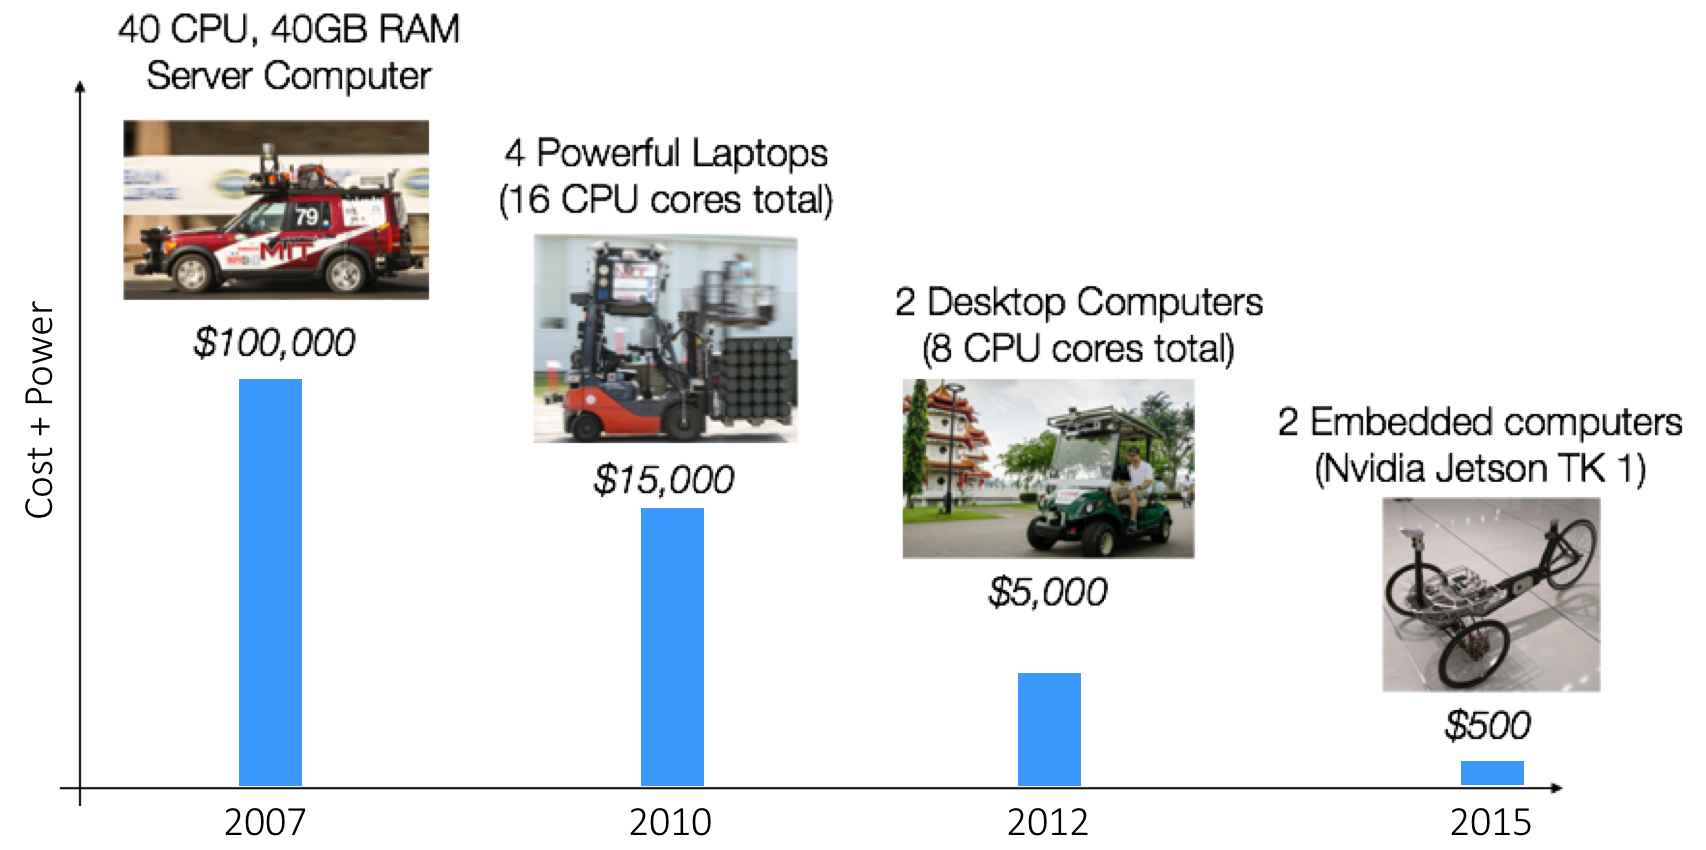
\includegraphics[width=\linewidth]{figs/01/computerCost2}
	\caption{The cost and the computational power required for self-driving cars has been greatly reduced during the last decade.}
\end{figure}

On the other side, throughout the last decade there has been an incredible decrease in the cost of computation time and in the size and power to process the data coming from the sensors. This point is critical in order to incorporate compact and affordable autonomy packages in current cars.

\begin{figure}[h]
	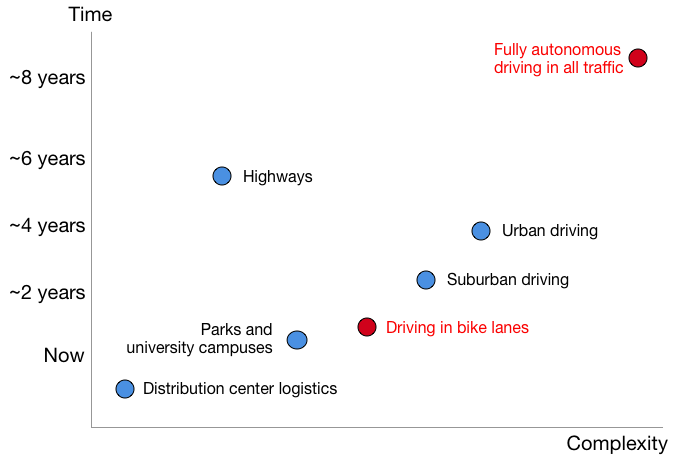
\includegraphics[width=\linewidth]{figs/01/autonomy_speed2}
	\caption{Challenges of self-driving vehicles based on the time of deployment and the complexity of the task.}
\end{figure}

However, achieving a level 5 of autonomy (based on SAE International Standard J3016\cite{SAEj3016}) will require years of development, due to the complexity of the task. Driving in bike lanes, on the contrary, makes up a straightforward challenge, basically because the road conditions and the sensors required for this task are not that demanding. The use of less and more affordable sensors will allow the deployment of intelligent three --or two in the future-- wheeler vehicles through bike lanes.

\subsection{Sharing Economy}

During the last couple of years, the sharing economy has disturbed the traditional way of moving in cities. Companies as \textit{Uber, Lift, BlaBlaCar, GetAround, Turo, Zipcar} and many others have offered a new way of commuting in urban areas. In this new paradigm, the technology has arrived to some countries without a proper regulation, which has caused complaints and protests from conventional transit services.
Other sectors, as housing (\textit{Airbnb}), goods (\textit{Wallapop}), food (\textit{LeftoverSwap}), sports equipment rentals (\textit{Spinlister}), and tourism (\textit{Vayable}) have also seen the irruption of this new way of economy.

More and more cities around the globe have adopted so called bike-sharing systems, which enable citizens and visitors to pick up bicycles at some point in the city, use them and leave them at another point in exchange for a small fee.

\newpage

\begin{figure}[t]
	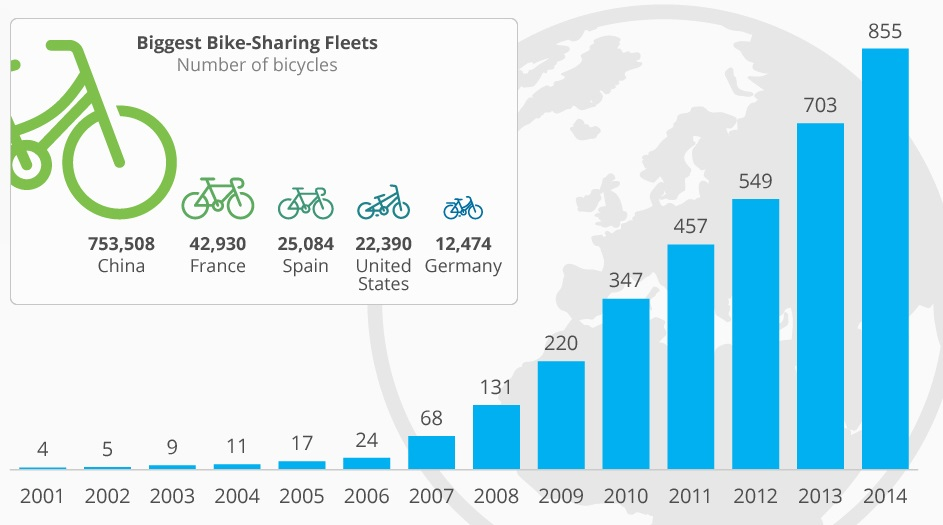
\includegraphics[width=\linewidth]{figs/01/Bike_Sharing_Systems_Worldwide}
	\caption{Number of cities worldwide that offer bike-sharing services. Source: \url{https://www.statista.com/chart/3325/bike-sharing-systems-worldwide/}}
\end{figure}




\subsection{Car-less Cities}

The ultimate policy will be to get rid of the vehicles in the city centers, as multiple cities have already announced.\cite{carFree} These can be seem as very radical strategies in transport policies, but the congestion and the pollution big cities are suffering at this moment exhibit much more issues and harm.

Therefore, is it possible to leverage electrification, autonomy and the shared economy to help fulfill this vision while ensuring a convenient flow of people and goods across the city?

%\newpage
\section{Persuasive Electric Vehicle}
Changing Places group\cite{cp} at MIT Media Lab\cite{ml} believes in the progressive fading of conventional cars from urban areas. The group's vision recalls on Kent Larson's\cite{kll} ideas, who affirms that the introduction of autonomous, electric and shared vehicles will hugely impact the cities of the future: Different streets layout, no more parking problems, less necessary vehicles and the overall result will be that the citizens will take the streets back from the cars. 

Furthermore, most trips in the city are one-person, low-speed, short distance. It does not make any sense to put one person in a 1800 kilograms vehicle to move across a city only a couple of kilometers. It was in front of this situation when the Changing Places group designed an ultra-lightweight one-person, three-wheel vehicle that is bike-like, not car-like.

\begin{marginfigure}
	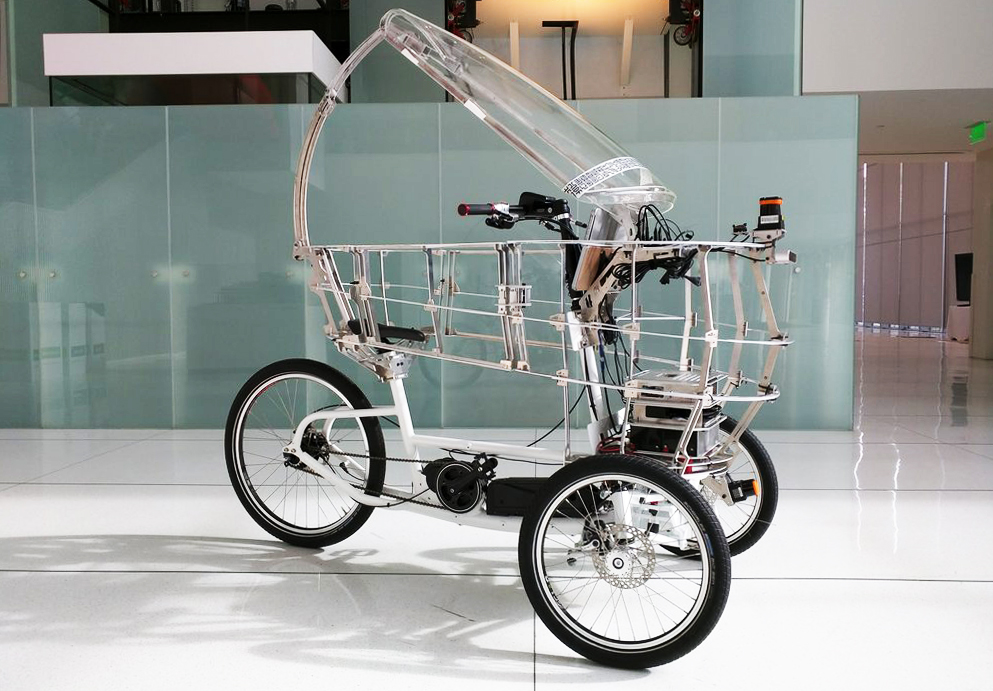
\includegraphics[width=\linewidth]{figs/01/pev_4}
	\caption{Persuasive Electric Vehicle (september 2016)}
\end{marginfigure}

\newpage
The \textbf{Persuasive Electric Vehicle}\cite{pev} (PEV) is an agile, on-demand, shared and functionally-hybrid tricycle with an expected contribution of 60\% emissions reduction and 30\% vehicle-distance reduction. The PEV is thought to constitute a new and indispensable category of vehicles in the emerging constellation of mobility systems. 

The PEV takes advantage of existing bicycle lanes, provides energy-efficient mobility, and addresses sedentary lifestyles. Designed with a cover to protect from the rain and the option for electric assist, PEV makes biking compelling for various demographics. 

Various \textbf{persuasive interventions} are displayed through user interaction with smartphones to facilitate pedaling behavior. Influential strategies are designed for both the interior and exterior of PEV. For example, an interior display shows how many previous riders have actually pedaled while riding a particular PEV. The exterior of the PEV changes color depending on whether a rider actually pedals or not.

\begin{figure}
	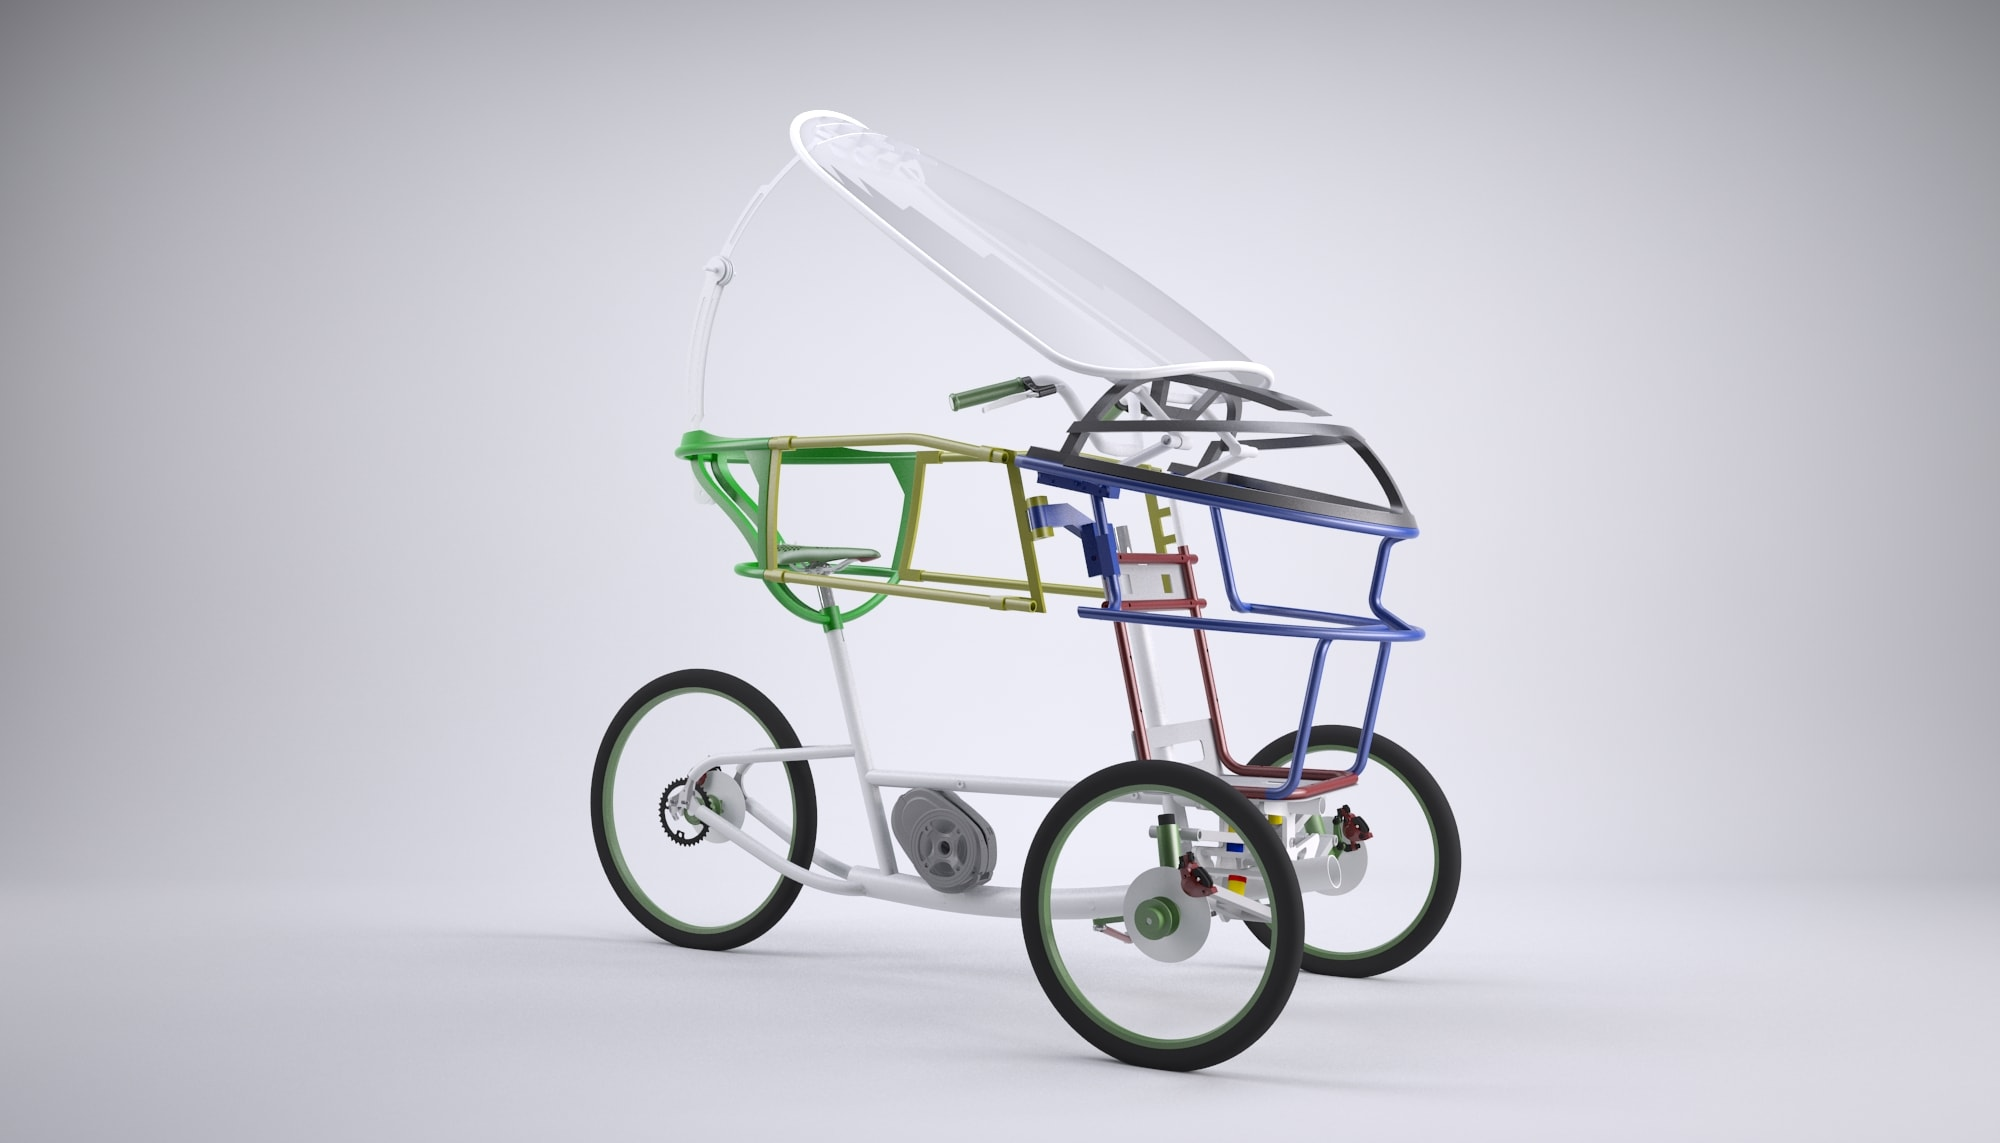
\includegraphics[width=\linewidth]{figs/01/pev_5}
	\caption{Persuasive Electric Vehicle render model}
\end{figure}

With a fabric exterior shield, a foldable canopy, and a 250-watt assist motor, the autonomous tricycle is "persuasive" in that it is designed to "encourage positive modal shifts in mobility behavior in cities." It has a top speed of 12 miles per hour, limited by the US regulation. It can be adapted for a human rider or for package transport, and it has the sensors and intelligence to operate autonomously.
 
\newpage
\subsection{Functionality}

-- \textbf{In transportation of goods} mode, the PEV will cover delivery on what is known as "the last urban mile". The PEV will be used as an autonomous courier service taking advantage of its attributes --small and maneuverable-- to efficiently service congested city areas even in cases of traffic cuts. 

\begin{marginfigure}
	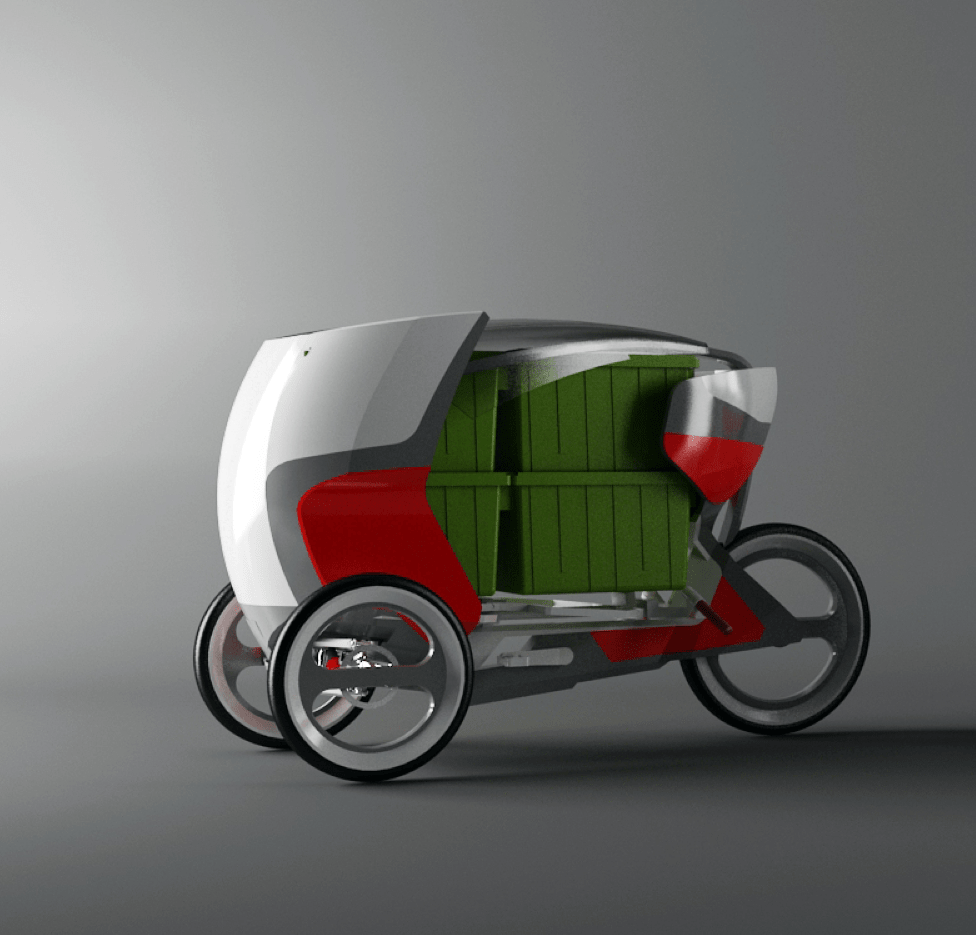
\includegraphics[width=\linewidth]{figs/01/folded}
	\caption{Logistics Mode PEV}
\end{marginfigure}

It could become a pervasive mode for urban package delivery, moving easily through crowded streets and reducing congestion and carbon emissions from gas-powered delivery vehicles.

-- \textbf{In passenger transport} mode, the PEV would function as a bicycle providing more safety and comfort thanks to its structural design, which offers more protection than conventional bikes, as well as its electrical assistance system, easing effort while pedaling.

Opposed to most shared bike systems, the PEV would "redistribute itself". Traveling autonomously from the drop-off point of one passenger to its next user's location, thus solving the problem of shortages and oversupply of bikes at different times in different locations. 

\begin{marginfigure}
	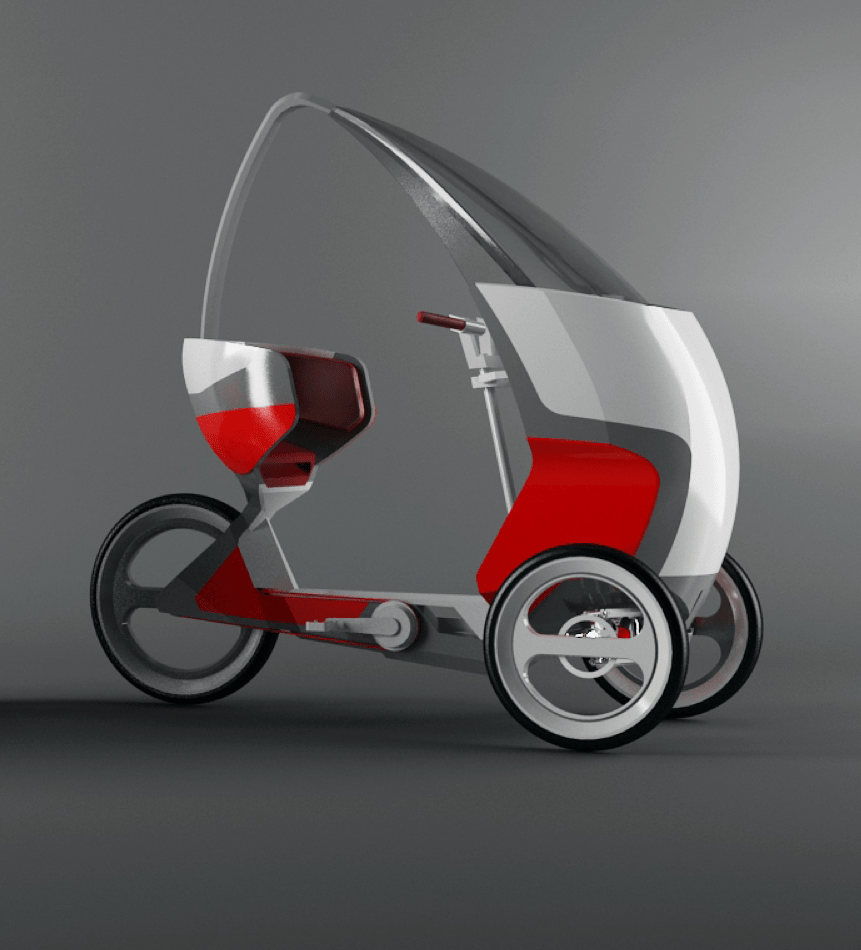
\includegraphics[width=\linewidth]{figs/01/unfolded}
	\caption{Passenger Mode PEV}
\end{marginfigure}

As for the \textbf{persuasive element}, studies show that those using ride sharing programs were already walking or riding their bikes more than others. Since the PEV is meant to expand the market for sustainable transportation, its focus is to give automobile drivers a reason to switch over-which is, a little exercise. By pedaling, riders generate energy that is stored up and used when needed by the motor. Passengers could choose to take care of their bodies, cities, and environment at the same time.

\subsection{Concluding Remarks}

The PEV is one of the upcoming new technological innovations that are set to change the way people commute in urban areas. Concerns over pollution and congestion of cities due to the increasing numbers of vehicles have seen man engage in inventions to improve their communities. Automobiles contribute largely to pollution; the development and use of the PEV would introduce an ecological mode of transportation. The elderly will also have reliable means of movement, which in turn encourage exercise and fitness.

\newpage
\section{Motivation}

The development of a new concept of intelligent vehicle opens the door to new research projects, in a \textbf{wide range of fields}. Computer vision, vehicle fleet simulations, persuasive technologies, mechanical design...are only few examples. Due to the open research opportunities, there is the necessity to understand in first place what people feel about the vehicle, from a user point of view. The conclusions of this analysis will narrow down the spectrum to this project's topic.

\subsection{Amazon Products Reviews}


A good way of understand the feelings of the people is to ask previous users about similar products. In this case, the most similar product was found in \textbf{adult tricycles}. The PEV's user demographics coincides with these vehicles users. Nowadays, one of the best databases of available user information can be found in Amazon\cite{Amazon}.

However, this information is not easily accessible. While it is true that Amazon used to provide access to product reviews through their Product Advertising API to developers and sellers, the company discontinued that on November 2010, preventing customers from displaying Amazon reviews about their products, embedded in their websites. As of now, Amazon only returns a link to the review.

Therefore, getting this data requires other methods. In this project, the dataset of Amazon reviews was downloaded using a \textbf{web crawler on the HTML} pages\cite{perl}. Given a first level domain ("com") and the list of IDs of Amazon products, this Perl script automatically downloads, from the Amazon server that is dedicated to that domain, all and only the HTML pages that contain the reviews about that products.

Another Perl script extracts all the reviews contained in the downloaded HTML files, outputting for each review a record with the following information:

\begin{itemize}
	\begin{itemize} \itemsep -15pt
		\item A counter of the extracted reviews
		\item Date of the review in \textsc{YYYY/MM/DD} format
		\item ID of the reviewed product
		\item Star rating assigned by the reviewer
		\item Count of "yes" helpfulness votes
		\item Count of total helpfulness votes ("yes"+"no")
		\begin{marginfigure}
			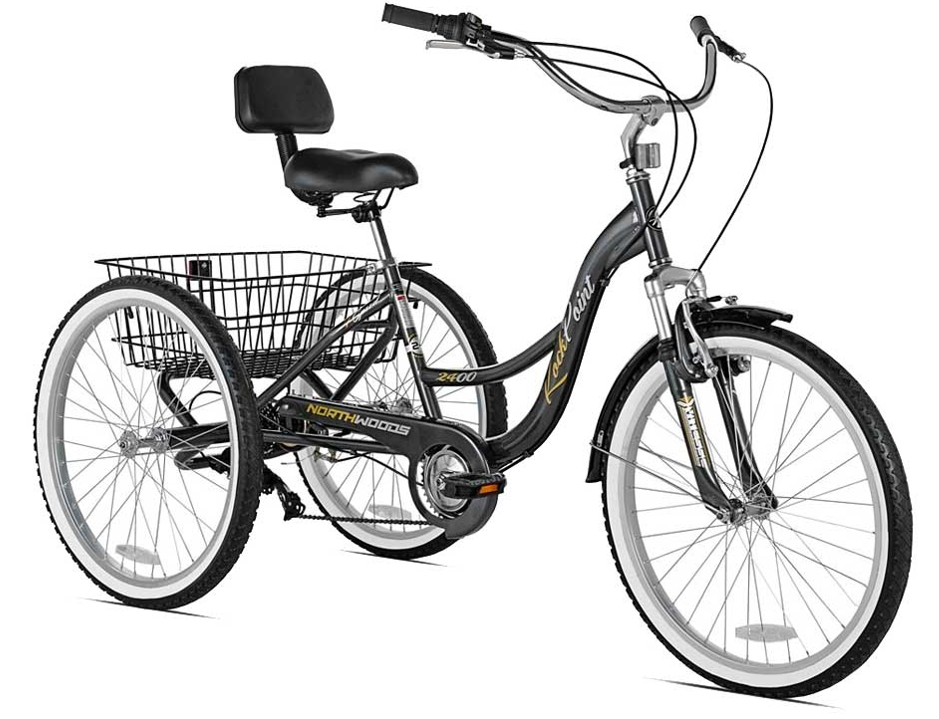
\includegraphics[width=1.2\linewidth]{figs/01/prodExample}
			\caption{One of the selected Amazon products}
			\label{prodExample}
		\end{marginfigure}
		\item Date of the review
		\item ID of the author of the review
		\item Title of the review
		\item Content of the review
	\end{itemize}
\end{itemize}

The selected products are really similar, with color, some components and accessories as main distinctions. The Figure \ref{prodExample} illustrates an example of one of the selected products, and more information has been included in Table \ref{productInfo}.

\begin{table*}[h!]
%\centering
\fontfamily{ppl}\selectfont
\label{productInfo}
\\[10pt]
\begin{tabular}{llc}
	\hline
	\textbf{Product ID} & \textbf{Product Description}  & \textbf{No. Reviews} \\
	\hline
	{B000IORU06} & Schwinn Meridian Adult 26-Inch 3-Wheel Bike           & 401\\
	{B000Z89JFO} & Kent Adult Westport Folding Tricycle                  & 157\\
	{B003F1WMZC} & Worksman Port-o-Trike Three Speed Adult Tricycle      & 42 \\
	{B00AWNI22I} & Schwinn Meridian Tricycle (26-Inch Wheels)      		 & 11 \\
	{B00FXMIUPW} & Mantis Adult's Tri-Rad Folding Trike					 & 2  \\
	{B00KDJC5UQ} & Komodo Cycling 24, 6-speed Adult Tricycle             & 2  \\
	{B00G3N5MZ6} & Torker 24 x 20 TriStar 2.1 Adult Trike 3 Speed        & 1  \\
	\hline
\end{tabular}
\\[15pt]
\caption{Detailed information about the analyzed Amazon products}
\end{table*}


Overall, over 670 reviews were extracted, being the Schwinn model the product with most of the reviews. Obtaining this information required a great deal of time, since Amazon does not like to have its web-page scraped, and the access gets banned, so a delay has to be introduced. This sleep delay starts with 5 seconds and increases over time, making really tedious to get the review data.

An alternative to this method would have been to use an already existing dataset. This option was studied, but it was not able to find any of the scoped products on the dataset, due to the available period of data (up to July 2014).

Having extracted the data, different approaches were implemented in parallel to understand the overall opinion of the users. In this way, it has to be pointed out that the review comments were predominantly too brief and that hardly expressed valuable ideas or details about the product. The majority of the users just valued the product from a very general perspective. Even with more than 670 reviews, the quality of the reviews could mislead the data analysis.

In the next section three analysis are explained, with their corresponding scripts included in the Appendices. I would encourage the reader to review the scripts after the following section, since the scripts include much more information and details while here brief explanations and the main conclusions are going to be explained.

%\newpage
\subsubsection{\textbf{Sentiment Prediction Analysis}}

\begin{marginfigure}
	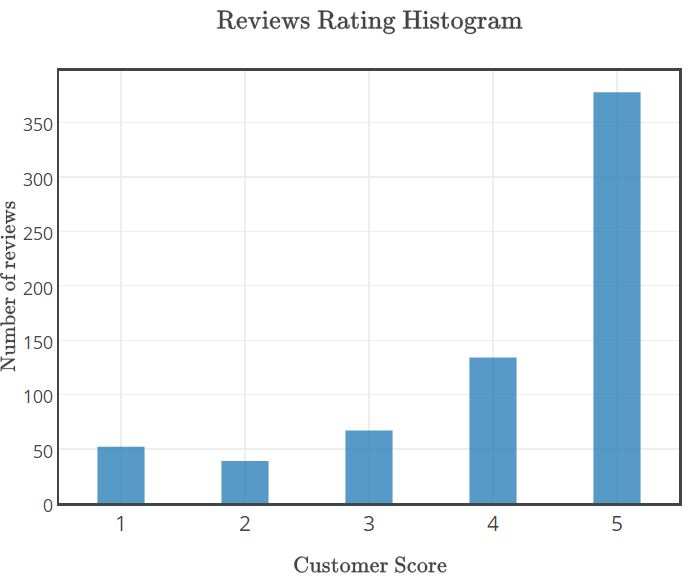
\includegraphics[width=1.3\linewidth]{figs/01/review_score}
	\caption{Reviews Rating Histogram}
	\label{starDistribution}
\end{marginfigure}

The purpose of this analysis was to investigate the positive and negative attitudes towards the selected products. Sentiment analysis attempts to determine which features of text are indicative of it's context (positive, negative, objective, subjective, etc.) and build systems to take advantage of these features.

Generally speaking, a satisfied customer will give 5 stars to the product, whereas few users will give poor evaluations (only if something really bad happened). This behavior is visualized in Figure \ref{starDistribution}, where the 5-star evaluation prevails.

This skewed distribution makes difficult to do a sentiment analysis based on the star-evaluation of the user. That is why the focus was not on the Score, but only in the positive/negative sentiment of the recommendation. Out of this analysis, the most positive and negative words are obtained:

\begin{figure*}
	\caption{Top 10 positive \& negative expressions and their score}
	\minipage{0.5\textwidth}%
	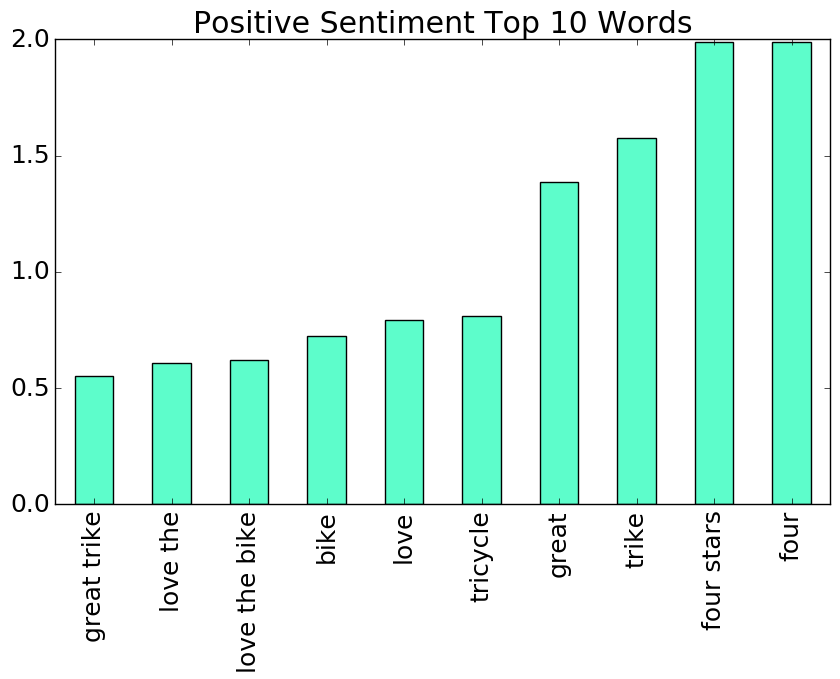
\includegraphics[width=1\linewidth]{pdf/Predicting_Sentiment_and_Helpfulness/Predicting_Sentiment_and_Helpfulness_files/Predicting_Sentiment_and_Helpfulness_13_2}
	\endminipage
	\minipage{0.5\textwidth}%
	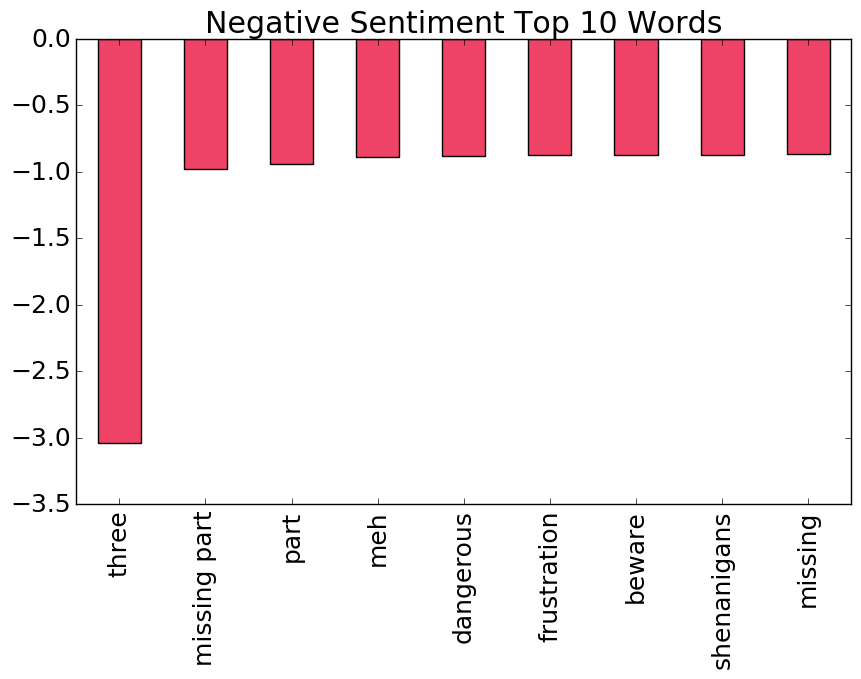
\includegraphics[width=1\linewidth]{pdf/Predicting_Sentiment_and_Helpfulness/Predicting_Sentiment_and_Helpfulness_files/Predicting_Sentiment_and_Helpfulness_13_1}
	\endminipage
	\\[6pt]
\end{figure*}

On the positive side, not much can be concluded, due to the lack on details. Customers that like the trike simply say it is a great product ("\textit{Four Stars}","\textit{Great},"\textit{Love}"), without saying why. This is totally opposite to the negative side, where much clear expressions appear.

\begin{table}[h!]
\centering
\label{most}
\begin{tabular}{cc}

	\begin{tabular}{c}
		\hline
		\textbf{Most Positive}\\
		\hline
		Four Stars\\
		Trike\\
		Great\\
		Tricycle\\
		Love \\
		Love the Bike\\
		Great Bike\\
		\hline
	\end{tabular}
	&
	\begin{tabular}{c}
		\hline
		\textbf{Most Negative} \\
		\hline
		Three\\
		Missing Part	\\
		Meh \\
		Dangerous\\
		Frustration    \\
		Beware		\\
		Shenanigans    \\
		\hline
	\end{tabular}
\end{tabular}
\\[10pt]
\caption{Selected relevant positive and negative expressions extracted from the sentiment analysis}
\end{table}

The main worries of the users are the missing parts from the trike and the danger or riskiness of the trike. The feelings of the user towards the product are summarized in "Meh" and "Frustration", both probably related to the assembly of the product. It also seems that the trike is dangerous to ride and that users should be aware of possible falls. For this project interest, one of these products weaknesses is starting to show up.

More information and the implementation of this program can be found in the
\hyperref[Predicting_Sentiment_and_Helpfulness]{\textcolor{blue}{Predicting Sentiment}} script on the Appendices.

\subsubsection{\textbf{Topic Modeling - LDA}}

Another way of analyzing the user data is to follow the topic modeling approach. By taking inferred topics and analyzing the sentiment of their corresponding documents (reviews) what customers are saying (or feeling) can be found. Examples from other authors\cite{bhatt2015amazon}\cite{chakankarsentiment}\cite{Mukherjee2012}\cite{rain2013sentiment}.

Latent Dirichlet Allocation (LDA) is the technique used to extract topics from Amazon reviews. It is assumed that there is some number of topics (manually chosen, 10 topics in this case), each topic having associated probability distribution over words and each document has its own probability distribution over topics. 

First, it scopes out a bunch of different \textbf{documents}, making note of the \textbf{words} in each of them. Crucially, it does not know the \textbf{topics} of each document, neither the different topics of each word.

Therefore, it picks some number of topics to learn, and starts by making a guess as to why each word belongs to each document. Of course, the random guesses are very likely to be incorrect, but there is a way to improve them, known as Gibbs sampling:
\begin{itemize}[noitemsep]
\begin{itemize} [topsep=6pt]
\item Go through each word $w$ in document $d$
\item For each topic $k$, computes two things: 
	\begin{itemize}
	\item p($k$|$d$) = the proportion of words in document $d$ that are currently assigned to topic $k$
	\item p($w$|$k$) = the proportion of assignments to topic $k$ over all documents that come from this word $w$. 
	\end{itemize}
\item Reassign word $w$ a new topic, where we choose topic $k$ with probability p($k$|$d$) * p($w$|$k$). According to the generative model, this is essentially the probability that topic $k$ generated word $w$.
\end{itemize}
\end{itemize}

\marginnote{
Specific Notation: \\
$\beta_{K}$ Topics\\
$\theta_{d}$ Topic proportions for document $d$ \\
$z_{d,n}$ Topic assignment for word $n$ in document $d$ \\
$w_{d}$ Observed words from document $d$ \\
$\eta,\alpha$, Dirichlet parameters \\
}
Finally it takes into account the distribution of each topic in each document (with the parameters $\alpha$ and $\eta,$ leading to:

\[p(\beta,\theta,z,w)=
\prod_{i=1}^K p(\beta_{i}) \prod_{d=1}^D p(\theta_{d}) \prod_{n=1}^N p(z_{d,n}|\theta_{d}) p(w_{d,n}|\beta_{1:K},z_{d,n})\]
 
 \begin{figure}
	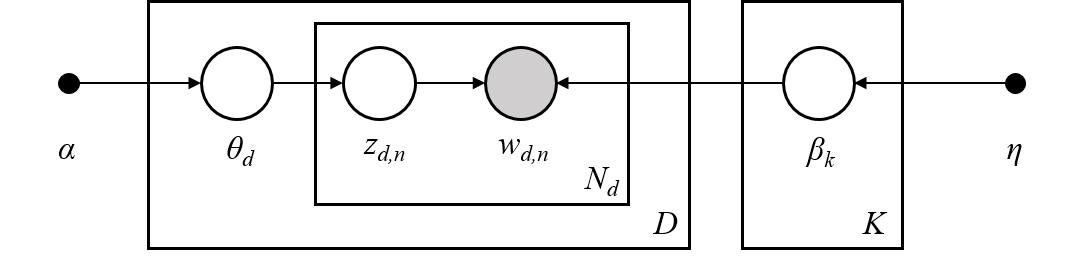
\includegraphics[width=1\linewidth]{figs/01/LDA}
	\caption{LDA graphical model. Boxes represent replicates. Outer box $D$ are documents, while inner box $N_d$ represents the repeated choice of words within the document}
	\label{LDA_graph}
\end{figure}

\newpage
Summing up, Gibbs sampling\cite{mcauley2015} basically takes some initial values of parameters and iteratively replaces those values conditioned on its neighbors (Figure \ref{LDA_graph}). Every word in all the text reviews is assigned a topic at random, iterating through each word, weights are constructed for each topic that depend on the current distribution of words and topics in the document, and we iterate through this entire process until it reaches a convergence.

All the reviews were converted to a bag of words and stop words removed. After the training of the model, a query was made passing a selected string to the model: "issues".

\begin{figure*}
	\caption{Results from the query to the LDA model: words from the most and less related topics}
	\minipage{0.5\textwidth}%
	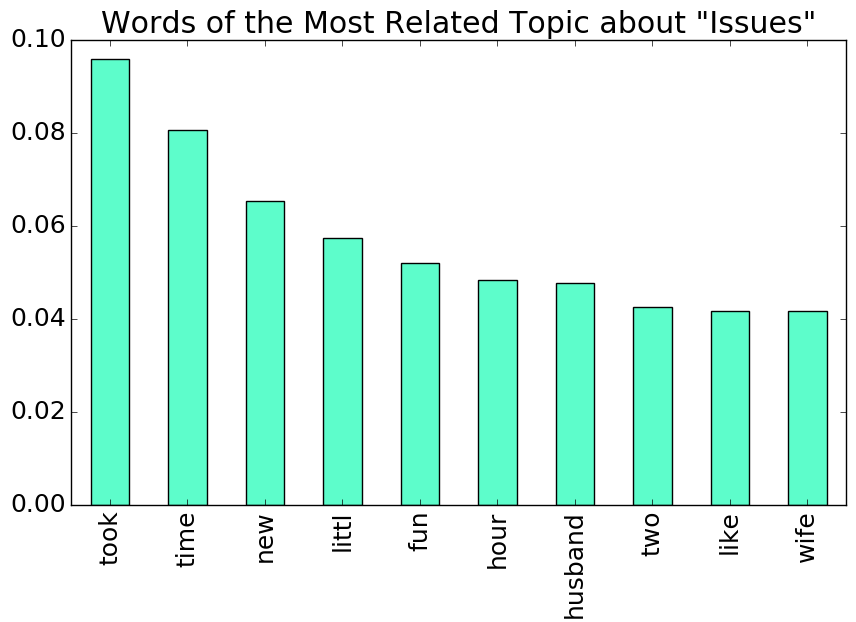
\includegraphics[width=1\linewidth]{pdf/Topic/Topic_Modeling_Amazon_Reviews_files/Topic_Modeling_Amazon_Reviews2_42_2}
	\endminipage
	\minipage{0.5\textwidth}%
	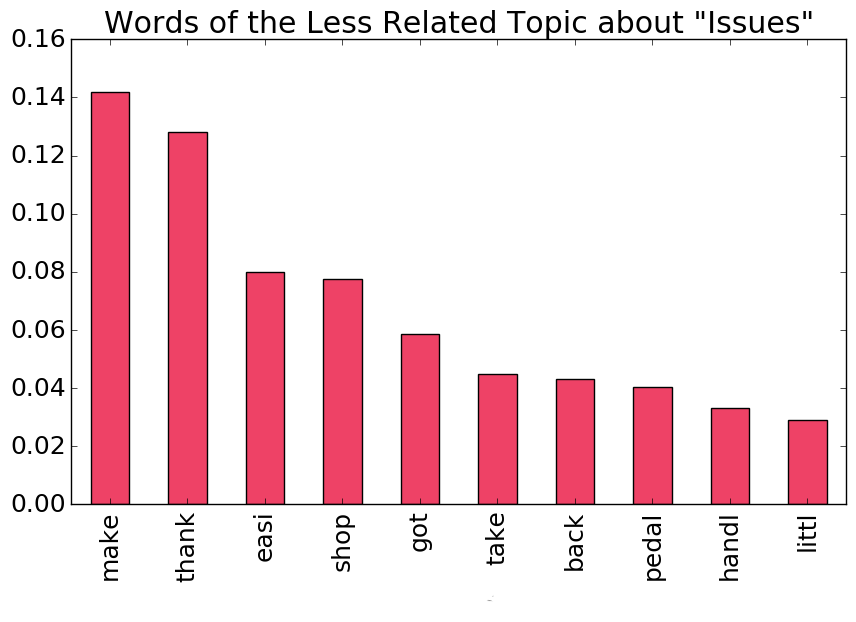
\includegraphics[width=1\linewidth]{pdf/Topic/Topic_Modeling_Amazon_Reviews_files/Topic_Modeling_Amazon_Reviews2_42_1}
	\endminipage
	\\[6pt]
\end{figure*}

The most related topic (0.66 correlation) talks about assembly issues, with words like "\textit{took}", "\textit{time}", "\textit{little}", "\textit{fun}", "\textit{husband}", "textit(wife)", whereas the less related topic (0.03 correlation)  contains ("\textit{make}", "\textit{thank}", "\textit{easy}", "\textit{shop}", "\textit{bak}"), which has little to do with any issues or problems. In fact, it seems this topic has not a clear meaning behind.
Fortunately, both topics do no share words, leading to the conclusion that these topics are far apart, and that are related to different aspects of the products.

As a conclusion to this analysis, the assembly of the bike (that comes in parts) supposes main problem to the users, an issue that will be out of the scope of this project. 

Overall, the results are not clear enough to to make an inference about their cause or origin. As the reader can notice, this analysis was not that successful, because the results could be interpreted in various different ways. Having only unigrams does not help to the interpretation of the results. That is why another way was approached, by means of keyword extraction and the wordcloud creation.

More information and the implementation of this program can be found in the
\hyperref[Topic_Modeling_Amazon_Reviews]{\textcolor{blue}{Topic Modeling}} script on the Appendices.

\subsubsection{\textbf{Wordcloud Creation}}

The Rapid Automatic Keyword Extraction (RAKE)\cite{rake} algorithm was implemented to easily extract keywords from the reviews, by identifying runs of non-stopwords and then scoring these phrases across the document. It requires no training, the only input is a list of stop words for a given language, and a tokenizer that splits the text into sentences and sentences into words.
 


A typical keyword extraction algorithm has three main components:
\begin{enumerate}\itemsep -10pt
	\item \textbf{Candidate selection}: extract all possible words, phrases, terms or concepts that can potentially be keywords.
	\item \textbf{Properties calculation}: For each candidate, calculate properties that indicate that it may be a keyword.
	\item \textbf{Scoring and selecting keywords}: All candidates can be scored by either combining the properties into a formula, or using a machine learning technique to determine probability of a candidate being a keyword. A score or probability threshold, or a limit on the number of keywords is then used to select the final set of keywords.
\end{enumerate}
	Finally, parameters such as the minimum frequency of a candidate, its minimum and maximum length in the words, or the stemmer used to normalize the candidates help tweak the algorithm's performance to a specific dataset.
	
\begin{marginfigure}
	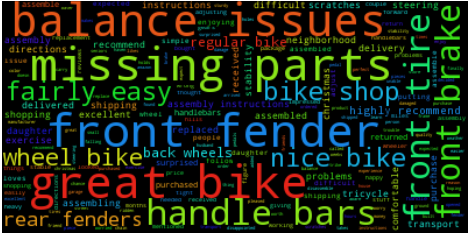
\includegraphics[width=1.2\linewidth]{pdf/Amazon/Amazon_clean_files/Amazon_clean_4_1}
	\caption{Unformated wordcloud of extracted keywords}
	\label{wordcloud1}
\end{marginfigure}
	
	In the Figure \ref{wordcloud1} there is the first version of the extracted wordcloud, without any format, and Figure \ref{wordcloud2} is the result after the formatting. The shape of the wordcloud was taken from one of the Amazon products, to simulate the form of a tricycle. More information and the implementation of this program can be found in the \hyperref[Amazon]{\textcolor{blue}{Wordcloud Creation}} script on the Appendices.
	
	From the wordcloud there were positive terms, as "\textit{great bike}", "\textit{front fender}", "\textit{fairly easy}","\textit{highly recommend}". Focusing on the negative features, some interesting terms appeared: "\textit{missing parts}", "\textit{rear fenders}", "\textit{bike shop}","\textit{balance issues}". Out of curiosity, these trikes do not have rear fenders but do have one in the front, leading to the users complains.

As a mechanical engineer, the term "\textit{balance issues}" was the one that attracted my attention. How can a three wheeler bike have balance issues? It is in fact intrinsically more stable than a bike, for sure. However, searching manually through some reviews, I noticed that the origin of this term was in some people complaining about falling when taking a curve, or one of the rear wheels lifting the ground. All these experiences made the users feel insecure when riding the trike. What could be done to avoid this problem?

\begin{figure}[t]
	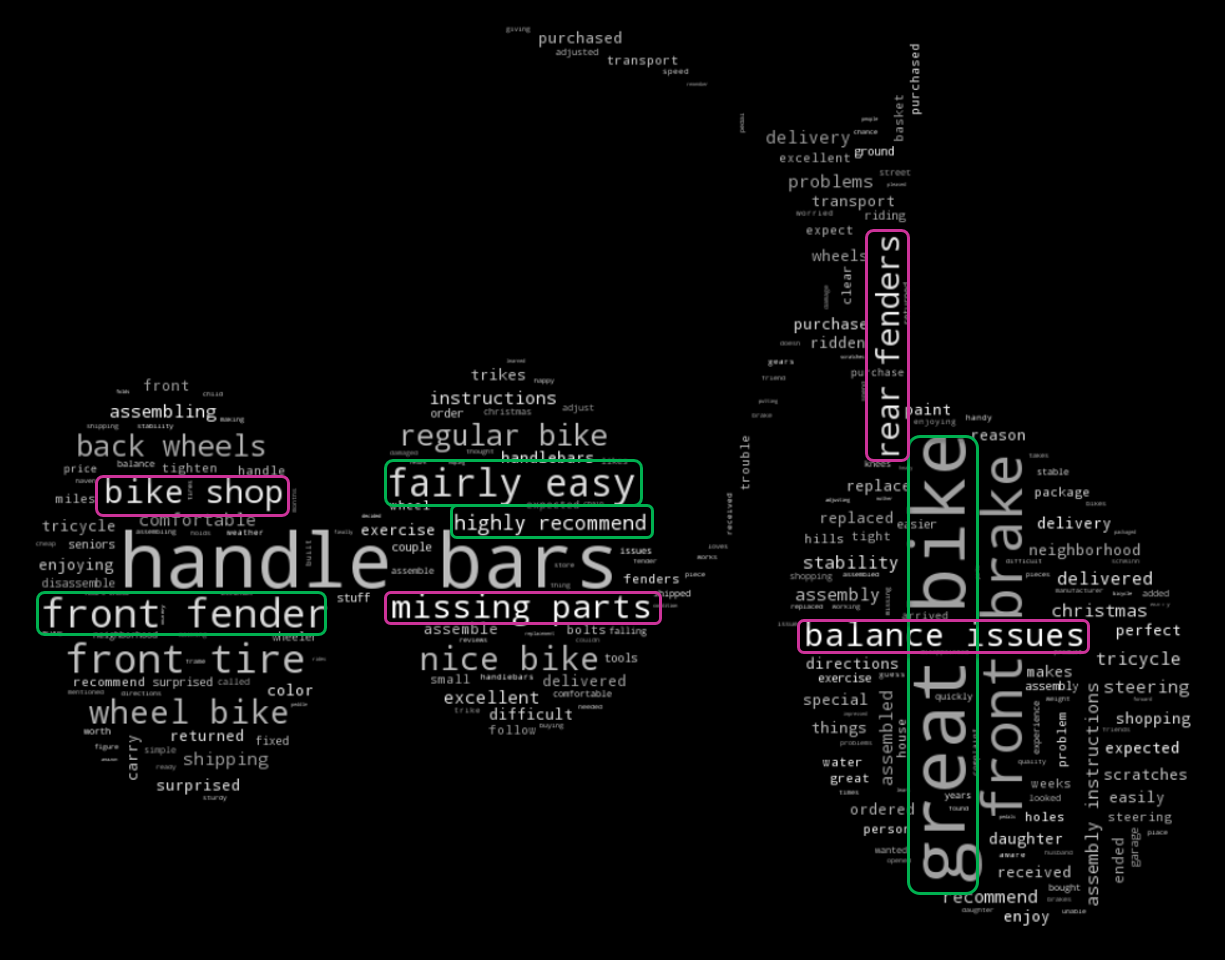
\includegraphics[width=1\linewidth]{pdf/Amazon/Amazon_clean_files/Amazon_clean_6_1}
	\caption{Formated wordcloud of extracted keywords}
	\label{wordcloud2}
	\\[-1cm]
\end{figure}

\section{Narrow Track Vehicles}

Balance or stability issues only appear when the user goes into a curve, otherwise the three wheels always support the trike in stable position. Let us analyze these type of vehicles in terms of the stability.

The PEV can be classified as a narrow track vehicle and, as it operates in normal driving conditions, it needs to be relatively tall to assure visibility. In Figure \ref{pevDim} the bounding box dimensions are represented. A tall narrow vehicle is characterized by a high centre of gravity to track width ratio, which makes vehicle \textbf{roll stability} an issue\cite{Saeedi}\cite{festini2011urban}.

When the track width of a vehicle is narrowed, there is an increasing in the the ratio of the center of gravity height with respect to the track width. This particular geometric property poses \textbf{stability problems for these types of vehicles while cornering}. Hence, such a narrow vehicle needs to be equipped with an inherent tilting mechanism that enables the vehicle to \textbf{tilt into turns while cornering}\cite{nurse2015tilting}. 

The added tilt degree of freedom should not require any stabilizing input from the driver. This brings about the need for an active control system that ensures the tilt stability (appropriate leaning during cornering) without affecting the handling of the vehicle.

\begin{figure}[t]
	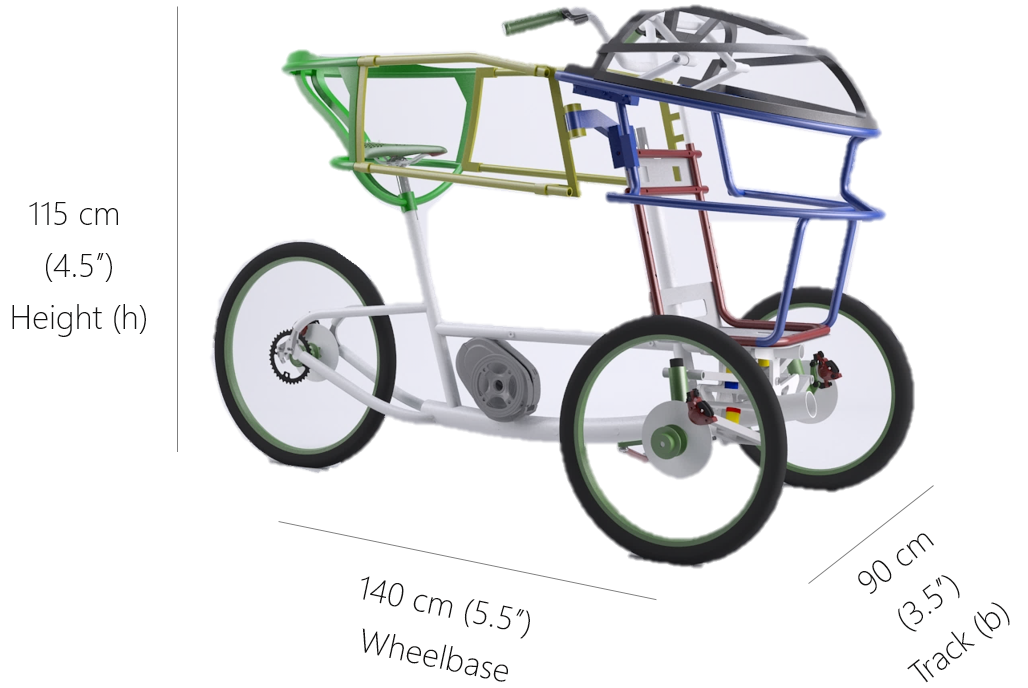
\includegraphics[width=1.0\linewidth]{figs/01/pev_6}
	\caption{PEV bounding box dimensions}
	\label{pevDim}
\end{figure}

Therefore, if such a vehicle is to negotiate curves through out its operating speed range, it needs to have a \textbf{capacity to tilt into the curve} like most two-wheeled vehicles. Consequently, an inherent tilting capability is required. 

This \textbf{tilting mechanism} should not require any special skills from the driver. The driver should be able to drive about as he/she would a regular four-wheeled vehicle. This, in turn, brings about a need for an \textbf{active tilt control system} that controls the tilting mechanism and ensures the stability of the vehicle and safety of the driver.

%\begin{marginfigure}
%	\centering
%	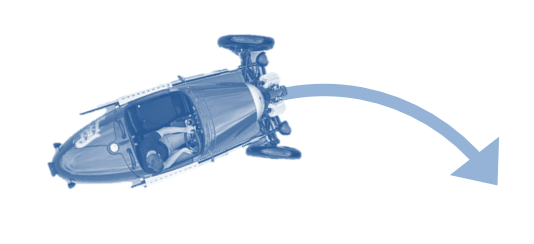
\includegraphics[width=1.15\linewidth]{figs/01/turn}
%	\caption{Right turn scenario for stability}
%	\label{turn}
%\end{marginfigure}

\subsection{Stability}

\marginnote{\\
$h_{g}$ Height of the center of gravity\\
$b$ Wheelbase width\\
$R_{l}, R_r$ Left and right wheel reactions\\
$F_y$ Lateral force\\
$T_{r}$ Moment due to the reactions $R_{l}, R_r$\\
$T_{f}$ Moment due to lateral force $F_y$\\
$m$ Mass of the vehicle\\
$g$ Earth gravity acceleration\\
}

Narrow vehicles that do not lean are unstable when they corner too hard. A simple statics calculation can illustrate this fact (Figure \ref{balance}).  

As the vehicle accelerates, for example, in a turn to the right, due to increasing lateral force $F_y$, the reaction in the right wheel $R_r$ approaches zero while the reaction in the left one $R_{l}$ approaches the weight force $mg$. 

At the balance limit, \[T_{r} = \frac{bmg}{2}\] and \[T_{f} = 2hF_{y}\]Overturning occurs if $T_{r} < T_{f}$, or similarly, the wheelbase is limited to \[b < \frac{4hF_{y}}{mg}\]By introducing tilt control, the \textbf{center of gravity is shifted} so that $R_r$ never reduces to zero. 

\begin{marginfigure}[-1cm]
	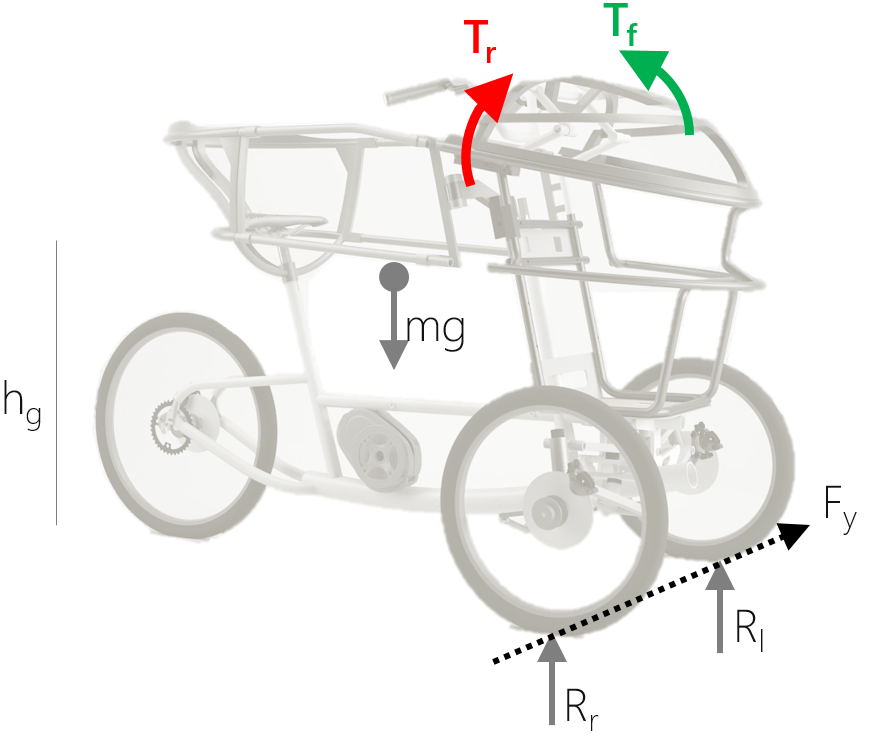
\includegraphics[width=1.3\linewidth]{figs/01/pev_7}
	\caption{Force schematic in a right turn scenario}
	\label{balance}
\end{marginfigure}

\newpage
\section{Research Objectives}

\begin{marginfigure}
	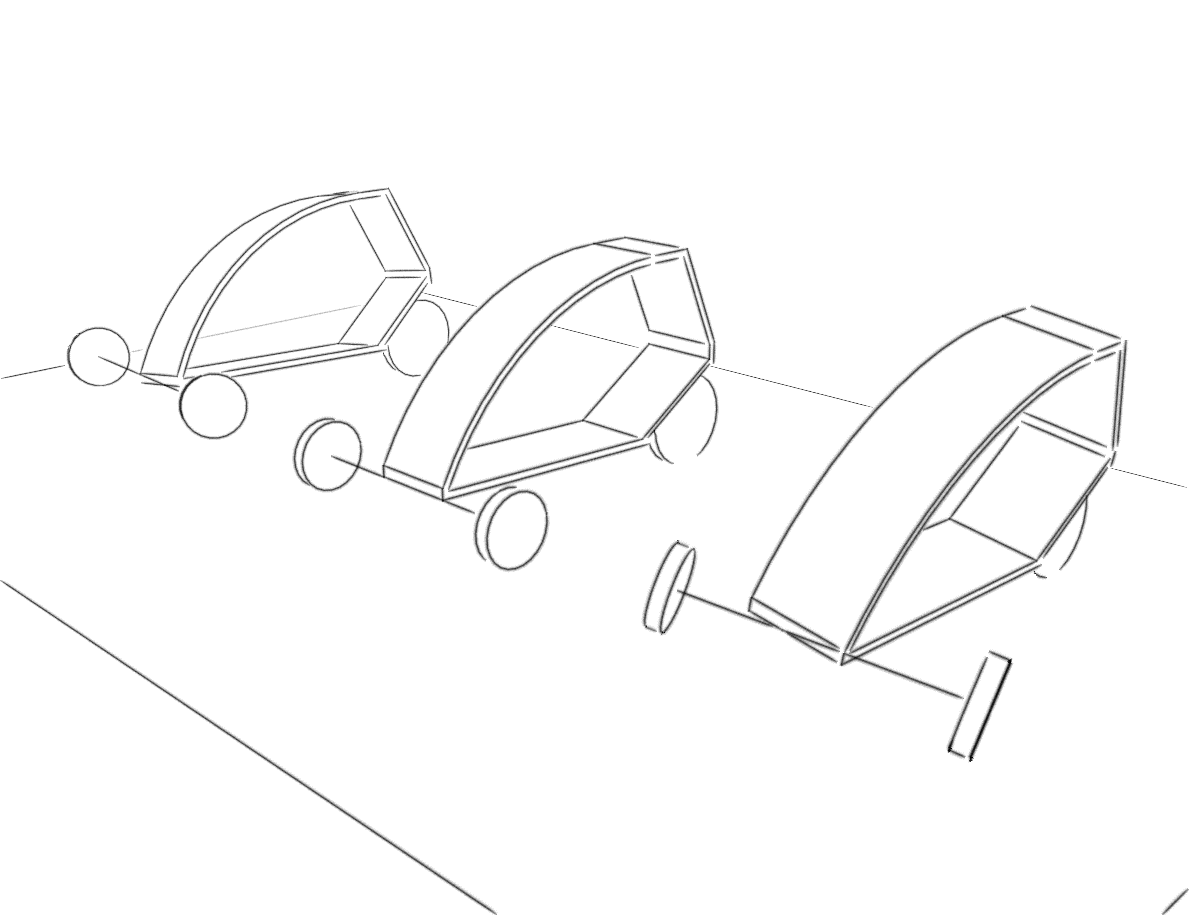
\includegraphics[width=1.3\linewidth]{figs/01/tilting_sketch}
	\caption{Simple first sketches of a tilting PEV}
\end{marginfigure}

This project is going to consist on the \textbf{design and fabrication of a three wheeler vehicle with an active tilting system}. The aim of the work presented here is summarized as follows:

\begin{itemize}\itemsep -8pt
	\begin{itemize}
	\item  The main objective was to \textit{design and fabricate a three-wheeled tilting vehicle} and to \textit{implement a roll control system}. In this way, due to the size, weight and cost limitations of a lightweight vehicle like PEV, it was critical to constrain the size of the motors and the feasible mechanical components.
	
	\item The first aim was to \textit{review the current developments} in vehicle modeling, roll control and tire modeling. Understanding the previous work in this field is fundamental to know the limitations and problems of the applied techniques. 
	
	\item The second aim was to implement and investigate models and methods to quantify uncertainties in the vehicle system such as the kinematics and environmental factors. These factors had a direct effect on the experimental results of road tests as well as the vehicle modeling and simulation. 
	
	\item The final aim was to set up an experimental test program to further the understanding of the dynamic model and the control of the three-wheeled tilting vehicle and to obtain data for the validation of the vehicle model.
	\end{itemize}
\end{itemize}

\newpage
\section{Thesis Structure}

This thesis consists of eight chapters and the following section outlines the structure of the chapters. 
\begin{itemize}\itemsep -8pt
	\begin{itemize}
\item \textbf{Chapter 2} reviews the literature relevant to all the aspects of this thesis: \textit{vehicle and roll dynamics modelling, roll control methods, driver modelling and tyre modelling}. The literature is critically discussed and a number of roll control methods, bicycle control strategies and rider models have been replicated. This chapter illustrates the status quo in the various research fields, highlights the gaps in the current knowledge. 

\item In \textbf{chapter 3} a \textit{linear vehicle model} is presented along with the proposed control method. It covers from the dynamic vehicle model to the calculations and simulations to test theoretically the control system. In order to improve the dynamic performance of the vehicle, \textit{linear optimal control theory} was used, and some design parameters for the control algorithm are presented.

\item \textbf{Chapter 4} explains the development of an small scale prototype of a tilting three wheeler vehicle. The components and design process are also documented in this section. 

\item \textbf{Chapter 5} presents the developed \textit{simulations to design the front suspension} and describes the \textit{fabrication process to build a real scale }tilting trike. The selected components and the electronic schematic is also exhaustively explained.

\item \textbf{Chapter 6} describes the application of the control strategy to the designed vehicle, as well as the \textit{experimental set up and the results from the carried out tests}. 

\item\textbf{Chapter 7} summarizes the \textit{materials, machining and labor cost} to carry out the project. 

\item Finally, \textbf{chapter 8} \textit{concludes the thesis} and presents a number of thoughts on future work.

	\end{itemize}
\end{itemize}
%For the background
%This brings up the main design criterion of the project. Instead of the driver balancing the vehicle as on a motorcycle, we desire a vehicle with an active tilt controller. The driver only performs lateral control to keep the vehicle in the road lane.
%
%An important consideration in any roll control design is the maximum moment limitation. Since the total of normal forces on both sides of the vehicle is in general equal to the weight, the limiting case will be when the entire weight of the vehicle is supported on one side.
%
%\[\abs{M_{x}}<M_{max}=\frac{mgb}{2}\]
